\documentclass[12pt,letterpaper]{article}
\usepackage[utf8]{inputenc}
\usepackage[spanish]{babel}
\usepackage{graphicx}
\usepackage[left=2cm,right=2cm,top=2cm,bottom=2cm]{geometry}
\usepackage{graphicx} % figuras
% \usepackage{subfigure} % subfiguras
\usepackage{float} % para usar [H]
\usepackage{amsmath}
%\usepackage{txfonts}
\usepackage{stackrel} 
\usepackage{multirow}
\usepackage{enumerate} % enumerados
\renewcommand{\labelitemi}{$-$}
\renewcommand{\labelitemii}{$\cdot$}
% \author{}
% \title{Caratula}
\begin{document}

% Fancy Header and Footer
% \usepackage{fancyhdr}
% \pagestyle{fancy}
% \cfoot{}
% \rfoot{\thepage}
%

% \usepackage[hidelinks]{hyperref} % CREA HYPERVINCULOS EN INDICE

% \author{}
\title{Caratula}

\begin{titlepage}
\begin{center}
\large{UNIVERSIDAD PRIVADA-DE-TACNA}
\vspace*{-0.025in}
\begin{figure}[htb]
\begin{center}

\includegraphics[width=8cm]{./Imagenes/logo}
\end{center}
\end{figure}
\vspace*{0.15in}
INGENIERIA DE SISTEMAS  

\vspace*{0.5in}
\begin{large}
TITULO:\\
\end{large}

\vspace*{0.1in}
\begin{Large}
\textbf{HERRAMIENTAS DE MAPEO OBJETO RELACIONAL (OR/M)} 
\end{Large}

\vspace*{0.3in}
\begin{Large}
\textbf{CURSO:} 
\end{Large}

\vspace*{0.1in}
\begin{large}
BASE DE DATOS II
\end{large}

\vspace*{0.3in}
\begin{Large}
\textbf{DOCENTE(ING):} 
\end{Large}

\vspace*{0.1in}
\begin{large}
 Patrick Cuadros Quiroga
\end{large}

\vspace*{0.2in}
\vspace*{0.1in}
\begin{large}
Integrantes: 
\begin{flushleft}
Orlando Antonio Acosta Ortiz		\hfill	(2015052775) \\
Orestes Ramirez Ticona              \hfill  (2015053236) \\
Nilson Laura Atencio     			\hfill 	(2015053846) \\
Roberto Zegarra Reyes 				\hfill 	(2010036175) \\
Richard Cruz Escalante 				\hfill 	(2013047247) \\
\end{flushleft}
\end{large}
\end{center}

\end{titlepage}


\tableofcontents % INDICE
\thispagestyle{empty} % INDICE SIN NUMERO
\newpage
\setcounter{page}{1} % REINICIAR CONTADOR DE PAGINAS DESPUES DEL INDICE

\section{¿Qué es un ORM?} 

\textbf{}\\
Hoy hablamos del Mapeo Objeto-Relacional o como se conocen comúnmente, ORM (del inglés Object Relational Mapping). Algunos de vosotros ya sabréis que son pero, para aquellos que no los conozcan, un ORM te permite convertir los datos de tus objectos en un formato correcto para poder guardar la información en una base de datos (mapeo) creándose una base de datos virtual donde los datos que se encuentran en nuestra aplicación, quedan vinculados a la base de datos (persistencia).

\begin{flushleft}

\begin{center}
	
	\end{center}
\begin{itemize}
\textbf{1.	Mapeo Objeto-Relaciona }
Si alguna vez has programado alguna aplicación que se conecta a una base de datos, habrás podido comprobar lo laborioso que es transformar toda la información que recibes de la base datos, principalmente en tablas, en los objetos de tu aplicación y viceversa. A ésto se le denomina mapeo. Utilizando un ORM este mapeo será automático, es más, será independiente de la base de datos que estés utilizando en ese momento pudiendo cambiar de motor de base de datos según tus necesidades.Veamos un ejemplo. Supongamos que tenemos una tabla de clientes. En nuestra aplicación queremos hacer las funciones básicas sobre base de datos CRUD (del inglés Create, Read, Update and Delete) Crear, Obtener, Actualizar y Borrar. Cada operación corresponde con una sentencia SQL.

\begin{center}
    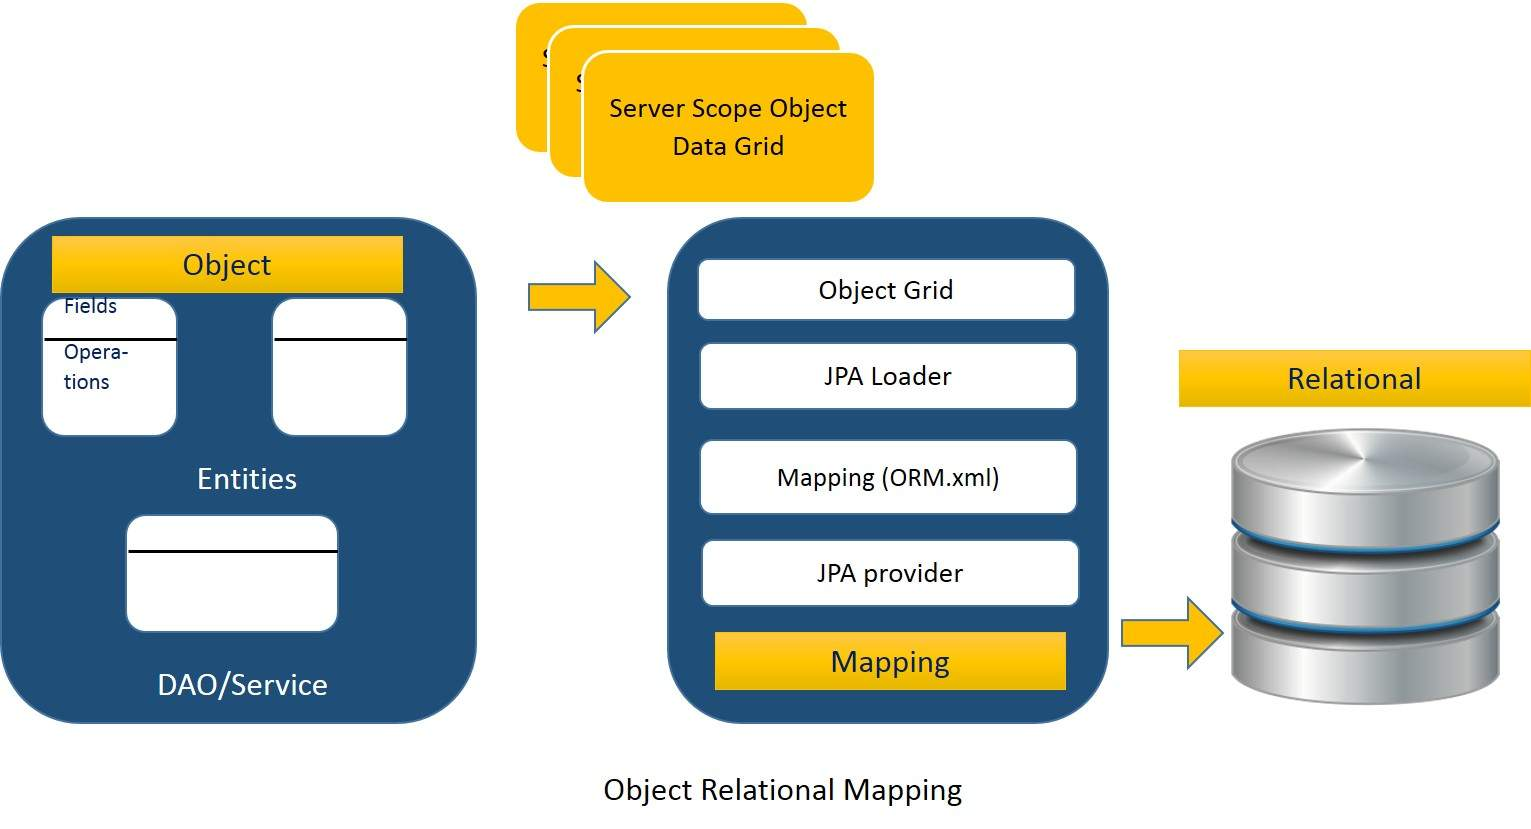
\includegraphics[width=12cm]{./Imagenes/map01}
    \end{center}


\begin{center}
El mapeo objeto-relacional (más conocido por su nombre en inglés, Object-Relational mapping, o sus siglas O/RM, ORM, y O/R mapping) es una técnica de programación para convertir datos entre el sistema de tipos utilizado en un lenguaje de programación orientado a objetos y la utilización de una base de datos relacional como motor de persistencia. En la práctica esto crea una base de datos orientada a objetos virtual, sobre la base de datos relacional. Esto posibilita el uso de las características propias de la orientación a objetos (básicamente herencia y polimorfismo). Hay paquetes comerciales y de uso libre disponibles que desarrollan el mapeo relacional de objetos, aunque algunos programadores prefieren crear sus propias herramientas ORM.



\textbf{}\\
\textbf{2. ORM (Mapeo Objeto Relacional)}

El Mapeo Objeto-Relacional es un técnica usada en programación para convertir los tipos de dato con los que trabaja un lenguaje orientado a objetos a tipos de dato con los que trabaja un sistema de base de datos relacional para la persistencia de datos. Básicamente consiste en una técnica que nos permite mapear cada una de las filas de nuestras tablas en la base de datos a objetos, en donde las columnas de la tabla corresponden a las propiedades de estos objetos.

Mientras que ORM es el nombre de la técnica, también se suele conocer como ORMs a los frameworks que la implementan, como EntityFramework en .NET, Hibernate en Java y ActiveRecord en Ruby. Estos ORMs usan convenciones de nombres, archivos de configuración en XML o anotaciones dentro del código para configurar la relación que existe entre una clase de nuestro lenguaje orientado a objetos y una tabla en la base de datos.

El uso de una herramienta de ORM introduce una capa de abstracción entre la base de datos y el desarrollador, ya que gracias a este mapeo, los ORM evitan que el desarrollador tenga que escribir consultas “a mano” para recuperar, filtrar, agrupar, eliminar, actualizar o insertar datos en la base, será tarea del ORM transformar las operaciones hechas a nivel orientado a objetos a sentencias SQL con las que la base de datos puede trabajar.problemas reales (por ejemplo, XML para el problema de intercambio de datos). - La empresa que desarrolla la herramienta deja de dar soporte a las viejas tecnologías y se centra sólo en las nuevas (por ejemplo, el soporte para OMT fue reemplazado por soporte para UML).

\end{itemize} 
\include{Secciones/Actividad02}
\include{Secciones/Actividad03}
\include{Secciones/Actividad04}
\include{Secciones/Actividad05}


\end{document}